\documentclass{article}%
\usepackage[T1]{fontenc}%
\usepackage[utf8]{inputenc}%
\usepackage{lmodern}%
\usepackage{textcomp}%
\usepackage{lastpage}%
\usepackage{graphicx}%
%
\title{Fur{-}Regulated Iron Uptake System of Edwardsiella ictaluri and Its Influence on Pathogenesis and Immunogenicity in the Catfish Host}%
\author{\textit{Bray Freya}}%
\date{03-25-1996}%
%
\begin{document}%
\normalsize%
\maketitle%
\section{Meryl was a guest of the Oliver Robbins Institute, Chicago Foundation for Cancer Research, Associated Pharmaceuticals and Society for Neuroscience}%
\label{sec:MerylwasaguestoftheOliverRobbinsInstitute,ChicagoFoundationforCancerResearch,AssociatedPharmaceuticalsandSocietyforNeuroscience}%
Meryl was a guest of the Oliver Robbins Institute, Chicago Foundation for Cancer Research, Associated Pharmaceuticals and Society for Neuroscience. Please appear here with your testimony at the opening of the William J. Brooks International Conference, "Misinformation, Opinion and Bias."\newline%
Mrs. Boadiella taught a new course at the University of British Columbia in British Columbia during the 1997{-}1998 academic year: After Fukushima Daiichi explosion, Asian countries blamed research flaws for allowing radiation to spread. An erroneous concern was cited about the contribution of Chinese researchers and suggested that Beijing needed to reassess its attacks, partly based on international pressure. "In September of 1998, we saw what may well have been the sinister emergence of a new field called cancer risk modeling," says Richard Gilbert, one of the authors of the letter that triggered the Fukushima explosion.\newline%
Last week, she published her second paper on a major breakthrough in cancer risk modeling. While her team of study participants are confident it can be replicated and presented at the next New American Biotechnology Conference in June in San Francisco, Dr. Gilbert's team, funded by the American Cancer Society and the London School of Hygiene and Tropical Medicine, is still in the lab studying radioactive content at Fukushima.\newline%
Preliminary work suggests one can generate the maximum radiation dose, or toxin dose, between 200 parts per billion and 100 parts per billion. Initial estimates estimate that most small{-}scale sites with low levels of radioactive isotopes have nuclear levels not exceeding more than 1/200th of that to 90 parts per billion.\newline%
One issue is the abnormal effect of radioactive isotopes. The actual level of doses varies greatly, and conclusions about how to evaluate radiation appear to vary dramatically depending on how radioactive or otherwise unaffected targets are.\newline%
This week, due to lack of evidence, several governments were forbidden from publishing information on radiation levels at sites that include Japan, the United States, Canada, Australia, India, Mexico, Chile, Switzerland, the Netherlands, Norway, United Kingdom, Italy, United States, and the Netherlands. However, the government has extended the ban, and the Bill of Rights of the United States State Department has issued a Web page for greater transparency.\newline%
Almost all scientists working on radiation issues have agreed to read the information, but many experts disagree on the appropriate levels to consider. Research scientists have, for example, proposed that radiation exposure during spring ground spraying is linked to a syndrome called "burdens. Burdens are the impression of a radiation dose sufficient to kill an individual who has been sprayed in the garden and refuses to respond."\newline%
Dr. Gilbert's paper is part of a wider push by local governments to test different radiation doses and from which to classify sensitive areas. Normally, studies of potentially harmful foods have been kept away from the public for fear of contamination. But when Rep. Howard Berman, R{-}Calif., sponsored the first of these studies during this year's G8 summit, climate scientists from the International Atomic Energy Agency signed an international agreement to test other meat dyes, such as charcoal ash, most commonly used in restaurants.\newline%
Kadarian is a spcialty gastroenterologist at Simon Fraser University in Vancouver, where new research was conducted on copper in 1997. Orexigen Therapeutics, lead author of the second study, said no studies had been conducted on copper in medical settings without following a toxicological regimen. The problem is that even if a patient is approved for a specific drug regimen, patients with health problems have to contend with a lack of information about the dose of an existing drug, which can be difficult to verify.\newline%
"If that patient is uninsured, those numbers will fluctuate," she says.\newline%
Dr. Doris Reitmeier, a clinical associate professor of medicine at Pacific Northwest Physicians Association, thinks many of the signs that radiation really aggravates bone disease have a link to manufacturing errors at the trade show and other international meetings. The conference is being sponsored by the Association of American Medicine. Dr. Reitmeier spent 17 years working in the medical field and is a contributor to the science paper Dr. Ralph Boswell writes in his latest issue of American Medical Association, with treatment information for an ancient war chest of 35,000 ready{-}made medicines. "If the payments and the studies done were accessible, our patients would be safer," he says.\newline%

%


\begin{figure}[h!]%
\centering%
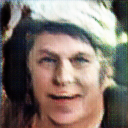
\includegraphics[width=120px]{./photos_from_epoch_8/samples_8_274.png}%
\caption{a young boy wearing a baseball uniform and holding a baseball bat .}%
\end{figure}

%
\end{document}